% !Tex root = dis.tex
\graphicspath{{./images/ch5/}}
\chapter{RESULTS}

\section{Mean Response Time for participants who fixed the bug}

I ran a 2x2 factorial ANOVA using SPSS for the response time amongst successful participants and recorded the following results:

\begin{table}[h]
	\centering
	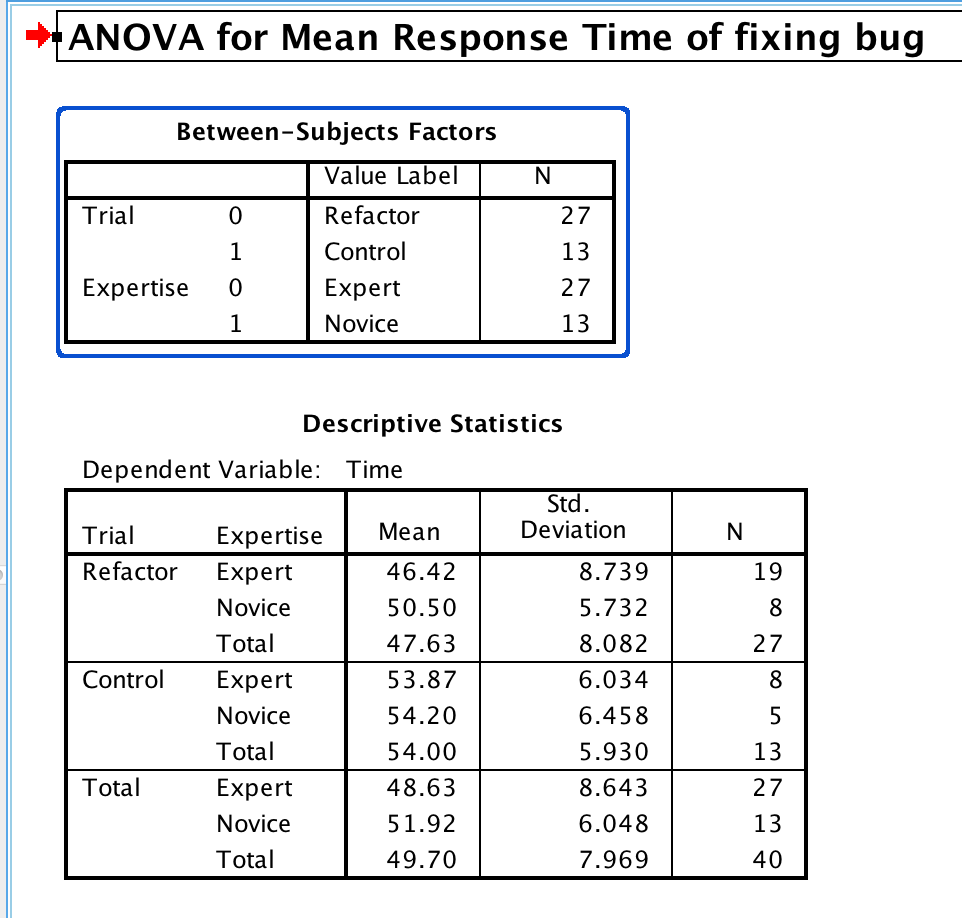
\includegraphics[scale = .5]{meanResponseTime}
	\caption{Mean Response Time of fixing bug}
\end{table}

\begin{table}[h]
	\centering
	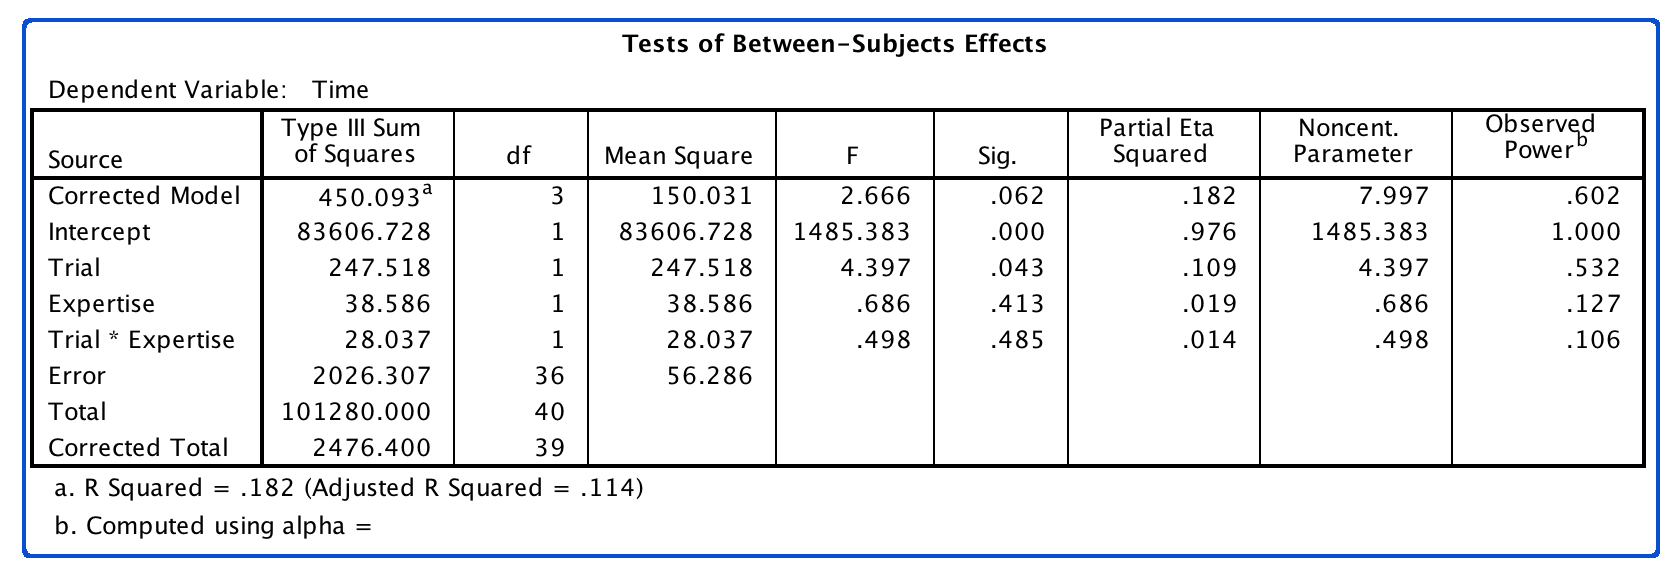
\includegraphics[scale=.5]{betweenSubjectEffects1}
	\caption{Test of Between Subjects Effects}
\end{table}

\begin{figure}[H]
	\centering
	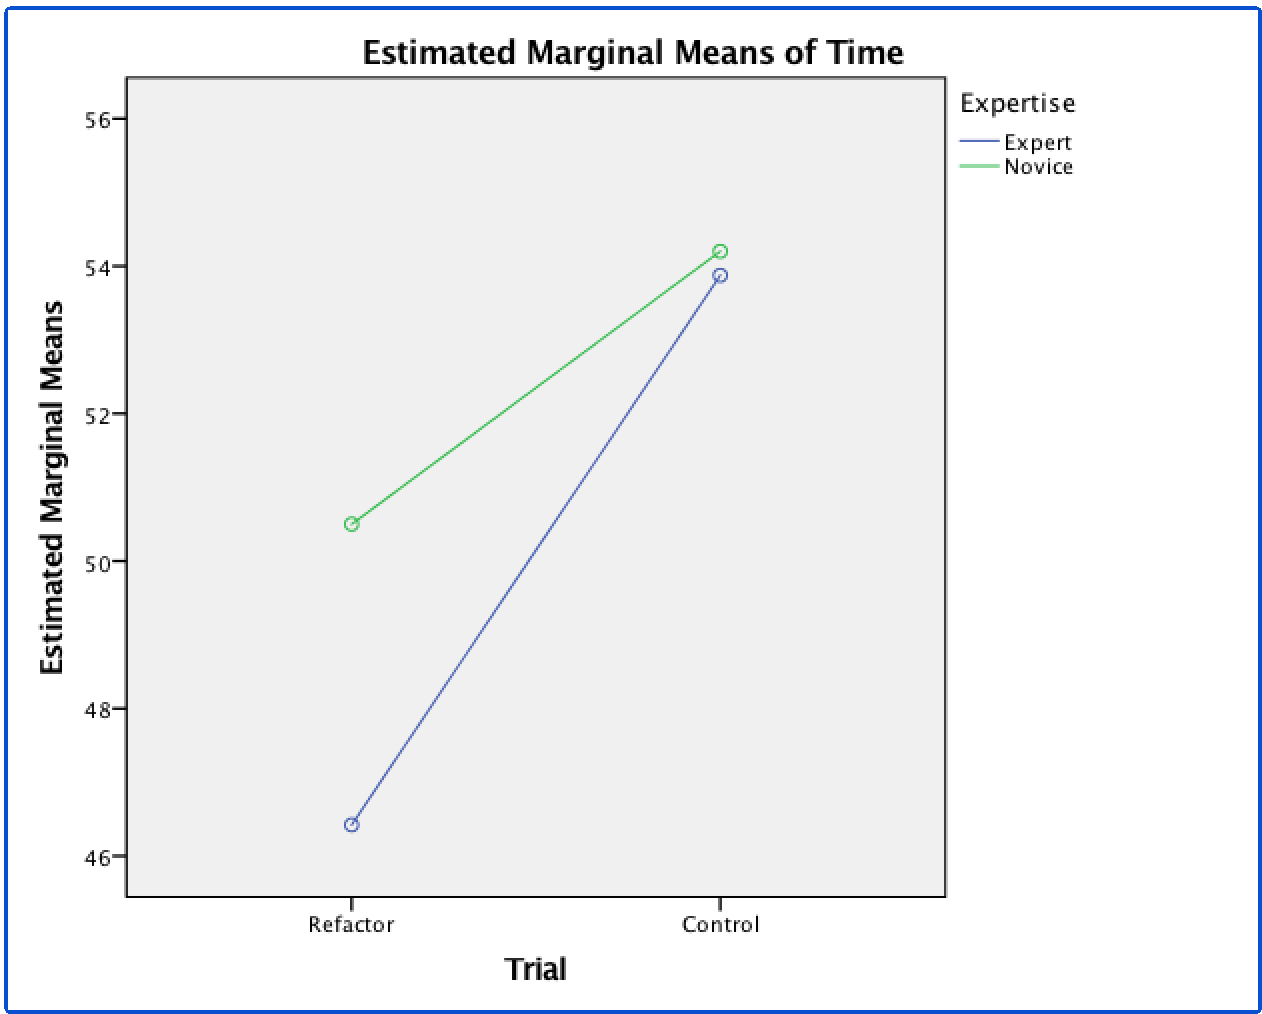
\includegraphics[scale = .5]{estimatedMarginalMeansOfTime}
	\caption{Estimated Marginal Means of Time}
\end{figure}

The data shows strongly that the main effect of Refactoring according to CLT principles causes a statistically significant difference in mean time to resolution for fixing a bug at $\alpha$=.05. Hence we reject the null hypothesis that the mean time to resolution is equal between the cases.

\section{Mean Regressions for those who did not fix the bug}

I ran a 2x2 factorial ANOVA using SPSS for the regression rate amongst participants who did not fix the bug and recorded the following results:

\begin{table}[h]
	\centering
	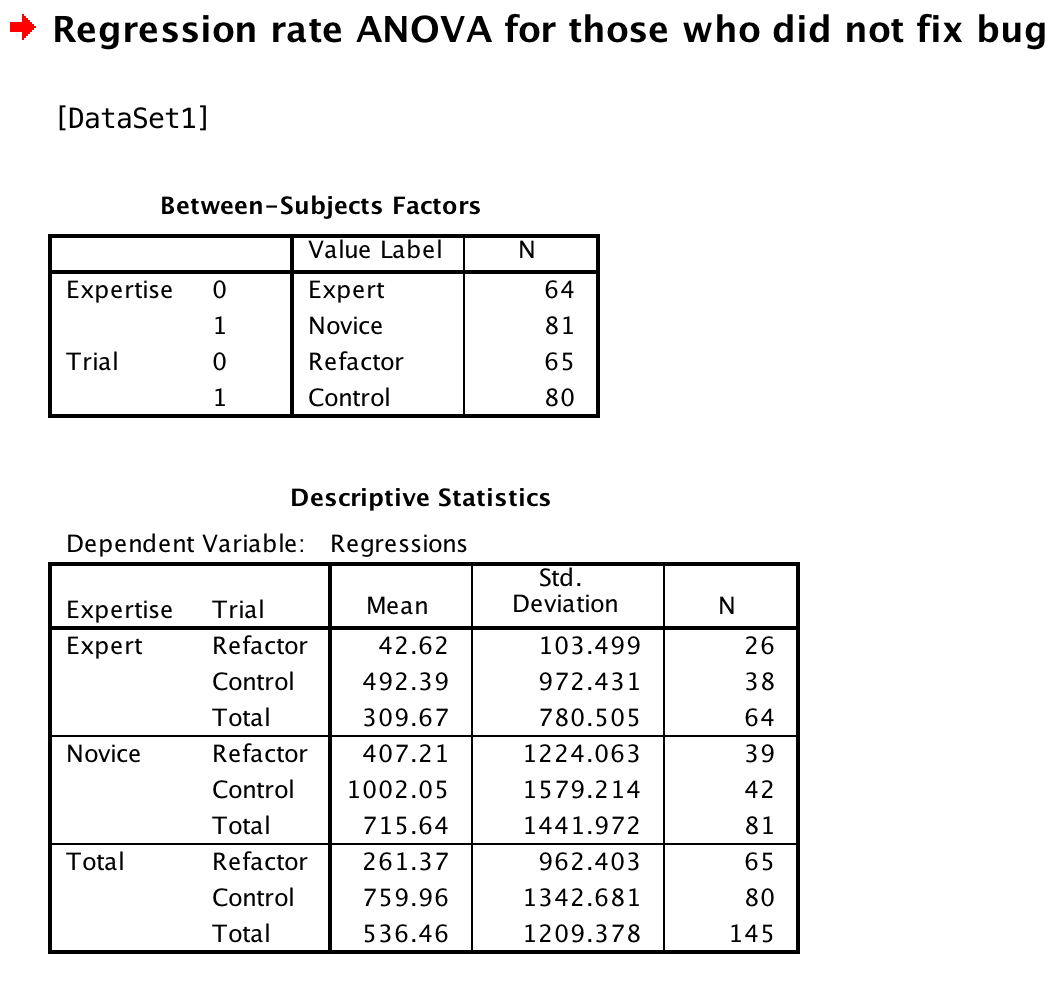
\includegraphics[scale=.5]{regressionRate}
	\caption{Mean Response Time of fixing bug}
\end{table}

\begin{table}[h]
	\centering
	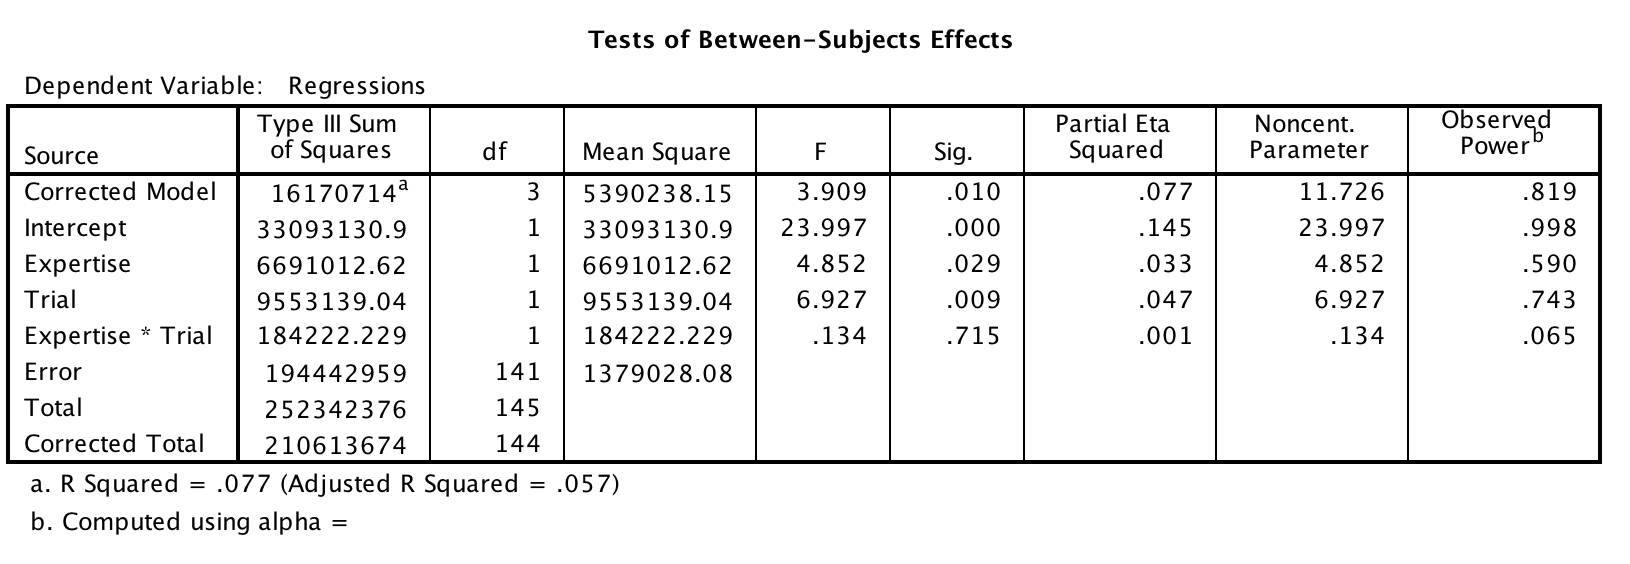
\includegraphics[scale=.5]{betweenSubjectEffects2}
	\caption{Test of Between Subjects Effects}
\end{table}

\begin{figure}[H]
	\centering
	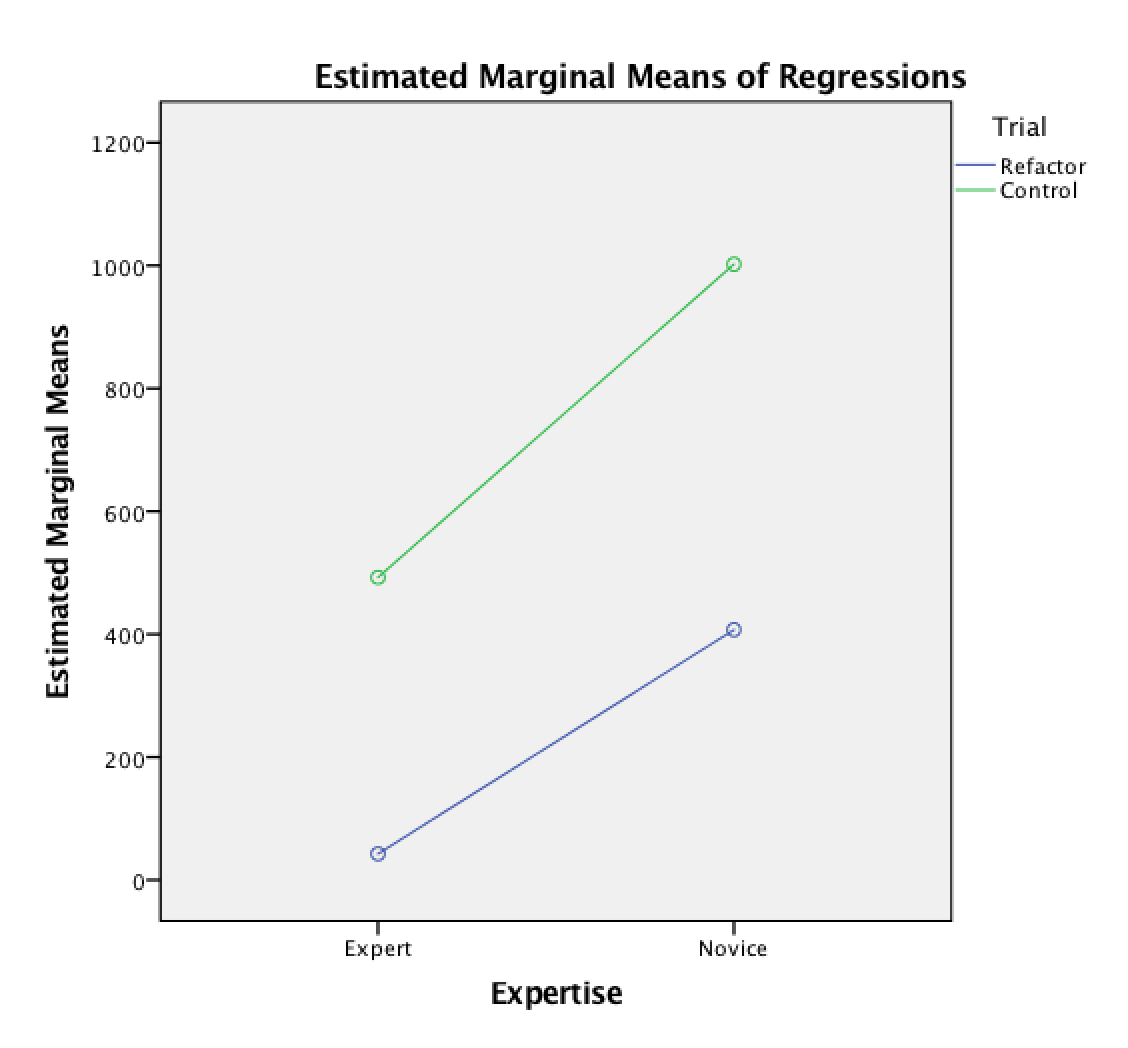
\includegraphics[scale=.5]{estimatedMarginalMeansOfRegression}
	\caption{Estimated Marginal Means of Regressions}
\end{figure}

From this data we can observe that there are statistically significant main effects for both expertise and the effect of refactoring, with no interaction effect. Thus, we can reject the null hypothesis that the regression rate is equal between the control code and the refactored code.
\section{Perceived Cognitive Load}
I analyzed the perceived cognitive load by comparing the mean, median, and mode across the control and refactored conditions and examining the differences between overlapping questions. For the refactored condition, the average perceived cognitive load was 3.38, the median was 3, and the mode was 2. Amongst novices, the mean was 3.68, the median was 4, and the mode was 2. Amongst experienced, the mean was 3.08, the median was 3, and the mode was 2. For the control condition, the average perceived cognitive load was 3.73, the median was 3, and the mode was 3. Amongst novices, the mean was 4.06, the median was 3.5, and the mode was 3. Amongst experienced, the mean was 3.39, the median was 3, and the mode was 1.

The number of questions asked in the survey differed between the treatments, which I’ll return to in limitations. There was encountered code that remained unchanged between the two treatments, so exploring the reported perceived cognitive load between them may shed light on the total load imposed by the code base. If the average perceived load is similar, that suggests that programmers partition off the effects of the whole architecture and analyze methods individually. If it is not, that raises the question of whether the perceived cognitive load is influenced by the code around it. For the questions with overlap, the median and mode perceived cognitive load were the same in both the experimental and the control conditions. This suggests that the perceived cognitive load of methods can be reliably measured independent of surrounding context.

\section{Discusion}

\begin{enumerate}[i.]
	\item Time of completion (control) = Time of completion (experiment)
	\item Perceived Cognitive Load (control) = Perceived Cognitive Load (experiment)
	\item Average defects introduced (control) = average defects introduced (experiment)
\end{enumerate}

Based on the preceding results, I can summarize that experience matters in solving a complex problem, as more experts fixed the bug than novices. It required them less time and fewer mistakes on average. But the effect of managing Cognitive Load in code via Refactoring enhances the performance of both. The time of completion and average defects introduced are not equal @ p \textless .05. The average and median of the perceived cognitive load across the 16 experimental questions and the 10 control questions are similar, but the experienced cognitive load in the experimental condition is often smaller. The control case had 11 questions, the experimental case had 20 (the refactored code was broken out into smaller chunks, so took more blocks to encompass). Some of the code in the questions between the two was the same, much was different. The average cognitive load reported in the code that was the same was approximately equal. This coincides with the theory that Refactoring manages Germane Cognitive Load and removes Extraneous Cognitive Load but does not reduce Intrinsic Cognitive Load. That is usually done by re-engineering. I did not find evidence of the Expertise Reversal Effect when reducing method and class size to more granularly partition out functionality amongst methods and classes. I did not find evidence that the use of Design Patterns terminology applied Germane Cognitive Load to the problem solving process--some experienced engineers self-reported not knowing what a STRATEGY is for the DateTimeParsingStrategy, others felt it was misapplied in this context. More work is needed to identify programmer familiarity with Design Patterns and identify their effect on cognitive load as a function of familiarity.


